\section{Wireless and Mobile Network}
Fino ad ora abbiamo trattato le reti con il presupposto che i nodi siano fermi nello spazio, negli ultimi anni tuttavia abbiamo assistito ad una vera e propria rivoluzione mobile.
La maggior parte degli host oggi giorno sono mobili, a partire dai dispositivi connessi tramite Wi-Fi, passando per quelli connessi a rete mobile di un qualche operatore telefonico, finendo per i cosidetti dispositivi IoT.
Si parla quindi di \emph{ubiquitous computing} cioè sistemi pervasivi talmente presenti da non farci neanche caso.

\subsection{Caratteristiche dei canali wireless}
Abbiamo diverse tecnologie wireless da quelle a corto raggio a quelle a lungo raggio, alcune caratteristiche sono:
\begin{itemize}
    \item la perdita di potenza del segnale: i segnali radio perdono potenza con almeno il quadrato della distanza

    \item interferenze da altre sorgenti: i collegamenti wireless sono molto più soggetti ad interferenze esterne e ci sono molte più sorgenti di interferenza
    
    \item multipath propagation: la propagazione del segnale può seguire diversi percorsi quindi un ricevitore riceve segnali uguali in tempi diversi, sfasati, bisogna quindi trovare il modo di non leggere un segnale arrivato tardi come un nuovo segnale
\end{itemize}
quello che ci interessa, dal punto di vista delle reti, è il bit error rate, questo dipende dalla codifica che decidiamo di utilizzare, non ce n'è una migliore in quanto ne esistono di veloci che però hanno un error rate alto e viceversa ne esistono di stabili ma lente.
I sistemi quindi sono di tipo adattativo cioè cambiano codifica in base alle condizioni del mezzo.

Il canale wireless è inoltre broadcast quindi è molto semplice che un host causi delle collisioni. Ci sono delle soluzioni a questo problema ma ne abbiamo alcuni altri.

\subsubsection{Problema del nodo nascosto}
Supponiamo di avere 3 ricetrasmettori: A, B e C e che:
\begin{itemize}
    \item A comunichi con B e viceversa
    \item B comunichi con C e viceversa
    \item A e C non possono comunicare perché hanno un ostacolo tra di loro oppure perché sono troppo distanti e l' attenuazione è troppa
\end{itemize}
quello che potrebbe succedere è che A e C comunicano allo stesso tempo, B riceve entrambi i segnali, c'è una collisione ma se ne accorge solamente B.
Pur facendo carrier sense A e C non possono sapere che c'è stata una collisione e non possono quindi attuare politiche di mitigazione.
\begin{figure}[H]
    \centering
    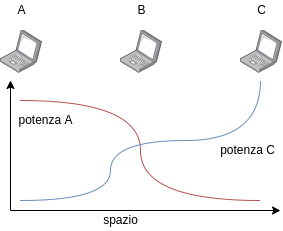
\includegraphics[width=250px]{images/8_Wireless_Mobile/wireless_attenuation.png}
\end{figure}

\subsubsection{Classificazione delle reti wireless}
Possiamo classificare le reti wireless in base alle dimensioni:
\begin{itemize}
    \item BAN: Body Area Network: pensate per reti di sensori indossabili, sotto il metro
    \item PAN: Private Area Network: pensate per piccoli dispositivi wireless con portata di qualche metro, ad esempio mouse, tastiere e dispositivi bluetooth
    \item WLAN: wireless LAN, le normali aree wireless per i computer
    \item Reti cellulari: reti GSM, GPRS, UMTS, LTE, ecc
\end{itemize}

Oppure in base alle infrastrutture:
\begin{itemize}
    \item reti basate su una infrastruttura: reti mobili.

    \item reti senza infrastruttura ad hoc: ad esempio reti formate da dispositivi bluetooth o le reti utilizzare da organi di pronto intervento che non possono fare affidamento su reti già esistenti.
    I nodi possono essere statici o mobili, possono essere multi-hop, possono poi essere connesse a delle reti pre-esistenti, ecc, ecc.

    \item reti ibride: reti con una porzione dotata di infrastruttura dedicata ed una porzione senza.
\end{itemize}

\subsection{Wireless LAN - 802.11}
E' lo standard de-facto per le reti wireless LAN meglio conosciute come Wi-Fi.
E' uno standard IEEE che ne raggruppa varie versioni in base alle frequenze ed altre caratteristiche.

E' un tipo di rete con infrastruttura, abbiamo quindi l' infrastruttura di rete fissa alla quale si aggiunge un \emph{Access Point} cioè una base station che si occupa di dialogare con i client wireless.
L' area di copertura è detta \emph{Basic Service Set} (oppure hotspot o cella).

Ogni host deve quindi associarsi ad un access point, spesso potrebbe ricevere il segnale di più di uno di essi e deve quidi scegliere quale usare.
Due access point adiacenti devono lavorare su canali diversi, cioè su frequenze di trasmissione diverse, ce ne sono 11 che occupano l' intero spettro che va dai 2.4GHz ai 2.485GHz.

\subsubsection{Associazione dell' host}
Quando un host vuole connettersi sceglie un canale e si mette in ascolto, esegue così la scansione di tutti i vari canali.
Gli Access Point ogni 100 ms inviano un beacon cioè un segnale che dice in broadcast il nome dell' access point (detto SSID) ed il suo indirizzo MAC.

Quindi l' host sceglie l' AP al quale associarsi, esegue eventualmente l' autenticazione necessaria, successivamente si configura in automatico con DHCP o in maniera statica ed è pronto a navigare.

\subsubsection{Accesso al mezzo}
Essendo il mezzo condiviso tra tutti c'è bisogno di un protocollo di accesso, potremmo pensare di utilizzare CSMA/CD tuttavia in questo ambiente non può essere utilizzato perché:
\begin{itemize}
    \item il dispositivo wifi se sta trasmettendo non può ascoltare il mezzo perché dotato di una sola antenna. Potremmo risolvere usando due antenne

    \item il problema del nodo nascosto persiste e non ci permette di detectare collisioni in quanto accadono sul nodo intermedio, non su chi sta trasmettendo.
\end{itemize}

Si usa un nuovo protocollo detto CSMA/CA (Collision avoidance) che si occupa di prevenire le collisioni, che tuttavia possono comunque accadere ancora.
Usiamo uno schema ARQ con una divisione in slot molto piccoli usati solo per dare il punto di inizio delle operazioni:
\begin{figure}[H]
    \centering
    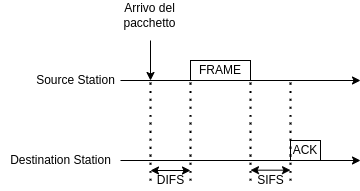
\includegraphics[width=300px]{images/8_Wireless_Mobile/802.11_comunication.png}
\end{figure}
\begin{enumerate}
    \item la sorgente vuole inviare un frame, il mezzo deve essere libero per un certo tempo che chiamiamo DIFS.

    \item se c'è stato DIFS tempo libero allora invia il frame

    \item subito dopo la ricezione del frame il destinatario muta da ricevitore a trasmettitore, questo tempo è detto SIFS (switching time) e deve essere necessariamente minore di DIFS.

    \item a questo punto il destinatario invia un ACK del pacchetto
\end{enumerate}
NB: SIFS $<$ DIFS perché altrimenti un altra stazione potrebbe inserisi nel mezzo ed inviare un frame causando una collisione.

Questa prima versione non tiene conto del fatto che potrebbero esserci più nodi in attesa di inviare: supponiamo ci siano due nodi che vogliono inviare, entrambi ascoltano il mezzo e misurano DIFS tempo libero, quindi trasmettono.
In questo scenario abbiamo certamente una collisione!
Per risolvere introduciamo un backoff time, ogni stazione oltre ad aspettare DIFS time ne aspetta altro randomicamente in modo da sparpagliare i tentativi.

Se mentre il timer di backoff ci si accorge che un' altra stazione inizia a trasmttere si congela il proprio timer e lo si risveglia dopo la fine della trasmissione e l' attesa del nuovo periodo DIFS.

Come tempo di backoff si sceglie un numero random di slot da aspettare in [0, CW-1].
Inizialmente CW vale cwim (standard del protocollo), quando si ha un ACK mancante si raddoppia CW fino ad arrivare a CWmax.

Questo protocollo tuttavia non ci risolve il problema del nodo nascosto: se i due nodi che vogliono comunicare non si vedono tra di loro ognuno vedrà il canale libero ed andrà a trasmettere causando una collisione in ricezione sull' access point.

Un altro problema che c'è è quello del nodo esposto: supponiamo di avere 4 nodi che parlano a due a due: B parla con A e C parla con D, D riesce a vedere solamente C.
Se B inizia a trasmettere verso A la stazione C non potrà trasmettere verso D in quanto troverà il canale occupato.
Se C non seguisse il protocollo e comunque trasmettesse potrebbe anche non causare problemi in quanto magari A è molto lontano da C, in questo caso si ha addirittura una perdita di tempo nell' attesa del canale libero.

E' stato quindi sviluppato un meccanismo detto \emph{virtual carrier sensing} che si contrappone al physical sensing perché anziché controllare la potenza del segnale per vedere l' utilizzazione del mezzo si esegue una specie di prenotazione del mezzo:
\begin{figure}[H]
    \centering
    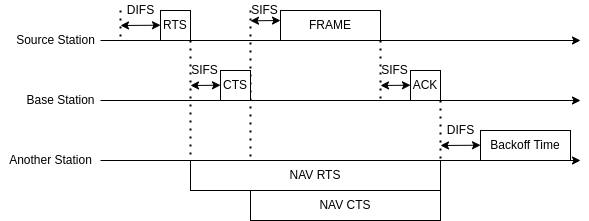
\includegraphics[width=330px]{images/8_Wireless_Mobile/virtual_carrier_sensing.png}
\end{figure}
Supponiamo ci sia una stazione che voglia trasmettere, allora guarda il canale e vede se è libero per un tempo DIFS, a quel punto invia un pacchetto RTS (request to send), viene ricevuto sia dalla stazione base che da tutte le altre stazioni vicini alla sorgente, chiunque senta questo pacchetto imposta un timer (NAV RTS - network allocation vector RTS) con la durata specificata nel campo \emph{duration} in RTS.
Successivamente dopo un tempo SIFS la base station risponde con un pacchetto CTS (clear to send) che contiene anche lui il campo \emph{duration}, con contenuto minore di quello trasferito dalla sorgente, ed è usato per far partire il timer (NAV CTS) a tutti gli altri nodi che non avevano sentito prima RTS.
Quando la sorgente percepisce il CTS (fa da acknowledge alla richiesta di trasmissione) aspetta un tempo SIFS ed inizia a trasmettere il frame.
Dopo la completa trasmissione del frame la stazione base attende un tempo SIFS ed invia un pacchetto di ACK.
Tutti gli altri nodi quindi vedono l' ACK e dopo un tempo DIFS fanno partire un timer di backoff con valore caricato randomicamente.

NB: se due host inviano RTS allo stesso tempo c'è ancora una collisione, tuttavia la grandezza di RTS è molto piccola quindi le probabilità di trasmissioni simultanee sono molto piccole ed anche se succedesse avremmo solo perso il tempo dell' invio di RTS.

NB: nonostante abbiamo risolto il problema c'è un aumento dell' overhead in quanto tutto il tempo dello scambio di RTS e CTS è tempo in cui non inviamo dati.
Per questi ed altri motivi se la grandezza del frame è paragonabile a quella di RTS/CTS non si esegue questo protocollo ma si invia direttamente il frame.

\subsubsection{Struttura del frame}
\begin{figure}[H]
    \centering
    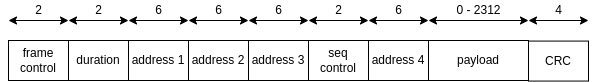
\includegraphics[width=330px]{images/8_Wireless_Mobile/802.11_frame.png}
\end{figure}
\begin{itemize}
    \item frame control: contiene informazioni di controllo sul frame
    \item duration: usato nei frame RTS e CTS per far settare i NAV alle altre stazioni
    \item address 1: indirizzo MAC della stazione che deve ricevere il frame
    \item address 2: indirizzo MAC della stazione che sta trasmettendo il frame
    \item address 3: indirizzo MAC dell' interfaccia del router al quale l' access point è collegato.
    E' utilizzato per trasformare il frame WiFi in un frame ethernet, questa traduzione è effettuata dall' access point che funziona un po' come un bridge.
    
    \item sequence control: numero di sequenza utilizzato per la ritrasmissione e l' acknowledge
    \item address 4: usato solo nella modalità ad hoc (quando una stazione comunica con un' altra senza l' ausilio di una stazione base)
    \item payload: i dati veri e propri
    \item CRC
\end{itemize}
il campo frame control a sua volta è costituito da:
\begin{figure}[H]
    \centering
    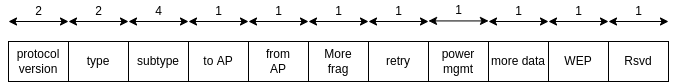
\includegraphics[width=330px]{images/8_Wireless_Mobile/802.11_frame_control.png}
\end{figure}
\begin{itemize}
    \item protocol version
    \item type: RTS, CTS, ACK, Data
    \item subtype
    \item to AP: indica se il frame è diretto all' access point
    \item from AP: indica se il frame è proveniente dall' access point
\end{itemize}

\subsubsection{Mobilità nella stessa rete}
Con le reti wireless possiamo avere problemi di mobilità, cioè l' utente si sposta.
Se la mobilità è nell' hotspot dell' access point allora non c'è nessuna modifica del funzionamento.

Se invece l' utente si sposta abbastanza da dover cambiare access point, ma comunque sempre nella stessa sotto rete, i due access point si mettono d'accordo e c'è una procedura di sgancio da uno ed aggancio all' altro.
Lo switch al quale gli access point sono associati potrebbe non capire che c'è stato un campio di topologia, quindi finché la tabella ARP non viene flushata l' host non riceverà i frame, dato che però il flush avviene molto spesso questo non è un problema.

\subsubsection{Power managment}
Essendo ora i dispostivi mobili è normale che vengano alimentati tramite batterie, quindi sarebbe bello prevedere all' interno dei protocolli di trasmissione dei metodi per risparmiare energia elettrica.
L' access point emette dei beacon ogni 100ms, come abbiamo già detto, sia per la discovery delle stazioni, sia per sincronizzare il clock, sia per le politiche di power management.

Quello che si fa è che i nodi vanno in sleep ed avvisano l' access point, a questo punto quando l' access point riceve frame che dovrebbero andare ad un nodo in sleep li mantiene in memoria ed aspetta che il nodo si risvegli prima di inoltrarli a lui.
Quando il nodo si risveglia ed effettua la sincronizzazione tramite il beacon con l' access point esso ne approfitta inviando la lista dei frame in coda.

C'è un piccolo delay quindi (sleep delay) perché bisogna aspettare che il nodo si risvegli, tuttavia c'è un grande guadagno in termini di energia preservata, si può ottenere fino al 90\% di efficienza.

\subsection{Architettura della rete mobile cellulare}
Questa rete è composta da alcune centraline che gestiscono un insieme di stazioni radio base.
Ogni smartphone si registra ad una stazione radio base e quindi si registra ad un centralino che poi è connesso alla rete intenet pubblica.

In origine la rete cellulare era una vera e propria rete telefonica tuttavia ormai anche la rete telefonica è stata convertita in una rete a commutazione di pacchetto.
Ogni stazione radio base viene detta cella quindi si parla appunto di reti cellulari.

NB: la forma esagonale è usata perché si disegna meglio, kek, in realtà sarebbero circolari.

Anche la rete cellulare essendo wireless è un mezzo broadcast quindi è necessario utilizzare protocolli che evitino le collisioni.
Per risolvere questi conflitti spesso si usano combinazioni di TDMA, FDMA e spread spectrum.

\subsubsection{Generazioni della tecnologia}
Ci sono diverse generazioni di questa rete cellulare, la prima era completamente analogica.

La seconda generazione, 2G, detta anche GSM combinava FDMA e TDMA era pensato solo per la voce ma era completamente digitale.
E' stata poi anche usata per trasmettere dati esattamente come si faceva con i modem casalinghi che sfruttavano la rete telefonica.

La seconda generazione e mezza, 2.5G, detta anche GPRS era una evoluzione del 2G che sfruttava sempre la stessa rete ma prendeva alcuni slot e li utilizzava esculsivamente per il traffico dati, rendendone più economico l' utilizzo.

La terza generazione, 3G, detta anche UTMS integra voci, video e dati in una singola rete.

La quarta generazione, 4G, detta anche LTE è completamente una rete IP sia per la trasmissione dei dati che per la trasmissione della voce.

La quinta generazione, 5G, pensata per applicazioni real time e mobili, quindi bassa latenza e pervasività.

\subsection{Mobilità in internet}
Internet è stata pensata per nodi stazionari e link affidabili (e wired), tuttavia l' evoluzione che ha preso non è stata questa.
Per alcuni versi la mobilità può essere gestita con soluzioni esistenti come il DHCP, tuttavia ci sono alcuni casi in cui questa gestione non basta per garantire la continuità del servizio.

\subsubsection{Mobilità per IP}
Dal punto di vista di IP la mobilità può essere:
\begin{itemize}
    \item nessuna: un host cambia punto di accesso alla rete ma rimane sempre nella stessa sottorete.
    Ad esempio un utente che cambia access point.
    In questo caso per il protocollo IP non ho cambiato punto di accesso, sono sempre nella stessa sottorete

    \item media: un host cambia rete acquisendo un nuovo indirizzo IP tramite il DHCP.
    Questa è mobilità ma senza continuità, non c'è da preoccuparsene

    \item alta: un utente si sposta da una rete all' altra in poco tempo, si ha ad esempio quando si viaggia ed il dispositio aggancia diverse reti man mano che ci si sposta.
    La continuità con la quale avvengono questi cambiamenti portano ad una situazione problematica e quindi è necessaria la gestione
\end{itemize}

Se per mantenere la continuità nel caso della mobilità alta dovessi disconnettermi e riconnettermi ogni volta che cambio indirizzo IP avrei un servizio intermittente.
Una gestione di questo caso non è previsto da IP, servono altre procedure ed altri protocolli.

\subsubsection{Indirect routing}
Una soluzione derivante da scenari del mondo reale prevede l' utilizzo di un \emph{home agent} che lavori per conto dell' host mobile.
Vediamo una situazione tipica:
\begin{figure}
    \centering
    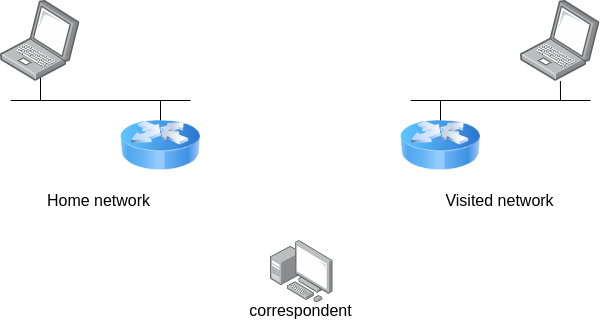
\includegraphics[width=250px]{images/8_Wireless_Mobile/mobility.png}
\end{figure}
supponiamo che l'host si trovi sempre nella home network ma a volte si sposti nella visited network, le due reti sono reti diverse con indirizzamenti diversi.
Chiamiamo il router della home network \emph{home agent} mentre chiamiamo il router della visited network \emph{foreign agent}.
Potremmo risolvere il problema attraverso i protocolli di routing annunciando che l' host si è spostato, tuttavia non è fattibile perché il routing funziona sulla base della rete e non del singolo host.

E' necessario che a gestire questa situazione siano direttamente gli host: quando l' host mobile arriva nella rete visitata, contatta il foreign agent e gli dice di registrarlo presso l' home agent.
Il foreign agent quindi contatta l' home agent avvisandolo che se dovessero arrivare dei pacchetti indirizzati verso l' host esso dovrà rispedirli al foreign agent perché l' host si è spostato.

L' host che quindi è all' altro endpoint della connessione (correspondent) non sa niente di questo cambiamento, continua e continuerà a spedire pacchetti a quello stesso indirizzo.
Quando l' host deve rispondere al correspondent invece può farlo direttamente.

Questo approccio funziona tuttavia c'è questa triangolazione del traffico che spesso è inutile e potrebbe essere evitabile, prende il nome di: triangolo del routing.
Questa soluzione è detta anche \emph{routing indiretto}:
\begin{figure}[H]
    \centering
    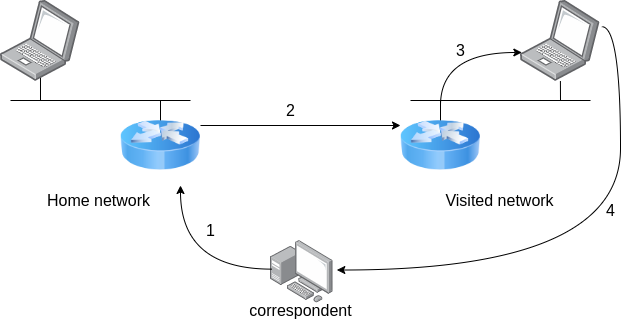
\includegraphics[width=250px]{images/8_Wireless_Mobile/indirect_routing.png}
\end{figure}
NB: l' home agent ed il foreign agent possono essere i router delle reti in cui l' host decide di spostarsi tuttavia non è obbligatorio.

NB: l' indirizzo IP orginale viene detto \emph{permanent address} mentre quello nuovo assunto una volta cambiata la rete viene detto \emph{care-of-address}.

Questo metodo è completamente trasparente al correspondent che non verrà mai a sapere che l' host si è spostato.

Si noti che se l' host si spostasse nuovamente esso dovrà nuovamente eseguire la registrazione presso l' home agent, in questo periodo la connessione non è presente, se quindi l' host è molto mobile si rischia di impiegare più tempo nel processo di registrazione che nella vera e propria navigazione.

\subsubsection{Direct routing}
Per risolvere il problema della triangolazione potremmo usare la tecnica del direct routing cioè quando il correspondent invia il datagramma all' home agent esso gli fa sapere che l' host si è spostato e gli indica anche dove.
In questo modo il correspondent può virare il suo traffico direttamente verso il foreign agent presso il quale si trova l' host mobile:
\begin{figure}[H]
    \centering
    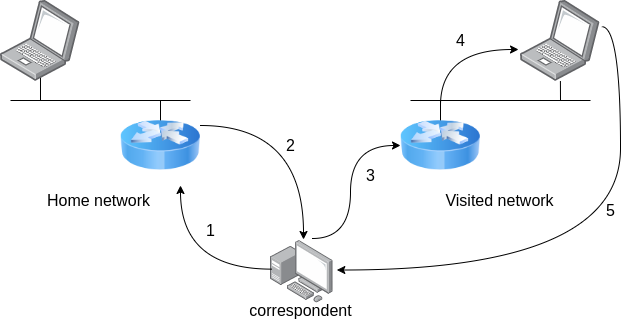
\includegraphics[width=250px]{images/8_Wireless_Mobile/direct_routing.png}
\end{figure}

Abbiamo eliminato la triangolazione del routing ma questo nuovo metodo non è trasparente rispetto al correspondent.
Se l' host mobile si sposta nuovamente in un' altra rete il correspondent continuerebbe ad inviare i datagrammi alla prima rete visitata, quindi è necessario che al nuovo spostamento l' host mobile si registri verso il vecchio foreign agent in modo che il correspondent possa essere avvisato del nuovo spostamento e dirotti ancora una volta il traffico verso la nuova posizione.

Per chi ha invece iniziato la connessione prima del secondo spostamento si ha una chain dei diversi foreign agent.

\subsubsection{Mobile IP}
E' un protocollo che usa l' approccio del routing indiretto, è descritto in RFC 3344 ed aggiunge il meccanismo di agent discovering e delle metodologie di registrazione verso l' home agent.

Quando l' home agent riceve un datagramma che deve instradare verso la nuova locazione dell' host mobile lo incapsula in un nuovo datagramma IP (inserendo come protocollo di layer superiore sempre IP, questo fa sì che questa incapsulazione possa essere eliminata all' arrivo senza particolari modifiche) e lo instrada.
Passa verso i foreign agent e viene recapitato all' host mobile.

L' agent discovery viene eseguito attraverso datagrammi ICMP trasmessi in broadcast dal foreign/home agent ad intervalli regolari:
\begin{figure}[H]
    \centering
    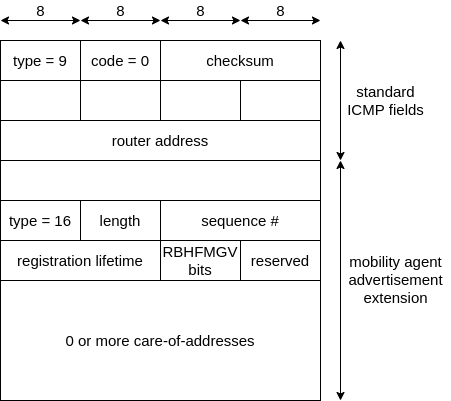
\includegraphics[width=330px]{images/8_Wireless_Mobile/agent_discovery.png}
\end{figure}
il pacchetto ICMP è di tipo 9 ed aggiunge dei campi specifici per gli utilizzi di discovery:
\begin{itemize}
    \item bit H/F: usati per indicare se è un home agent e/o un foreign agent
    \item bit R: indica se è necessaria la registrazione
\end{itemize}

La registrazione consiste di 4 passi: supponendo che l' host mobile sia arrivato nella nuova rete e che abbia correttamente ottenuto un indirizzo IP, allora
\begin{itemize}
    \item l' host mobile aspetta di ricevere un pacchetto ICMP per l' agent discovery, in questo pacchetto ci sono dei care-of-address offerti, ne sceglie uno e se lo assegna

    \item invia un messaggio al foreign agent in cui trasmettere:
    \begin{itemize}
        \item COA: care-of-address scelto
        \item HA: indirizzo dell' home agent
        \item MA: suo indirizzo corrente
        \item lifetime
        \item identificativo usato come numero di sequenza
    \end{itemize}
    
    \item il foreign agent riceve la richiesta di registrazione, memorizza i dati ivi contenuti e spedisce la richiesta all' home agent aggiungendo anche una nota sul tipo di encapsulation da usare.
    
    \item l' home agent riceve questa registrazione, segna le informazioni, abbassa il lifetime richiesto e risponde con un pacchetto di risposta identico a quello di registrazione ma togliendo il COA
    
    \item il foreign agent ottiene la risposta dall' home agent e la spedisce all' host mobile. Da questo momento in poi l' eventuale correspondent può inviare traffico e verrà instradato verso il mobile host.
\end{itemize}

\subsection{Effetti della mobilità sui protocolli di alto livello}
Logicamente l' impatto dovrebbe essere minimo tuttavia data la natura di TCP, che vede nella perdita di pacchetti una congestione, si ha una forte diminuzione della performance.
Questo è vero anche se si ha a che fare con collegamenti wireless o in genere con collegamenti che possono avere delle perdite.

Quello che si fa per non perdere performance nel caso delle reti wireless è gestire la perdita di pacchetti a livelli più bassi quindi tramite schemi ARQ prima di far arrivare i dati al layer TCP.

Un' altra opzione è quella di rendere noto al layer TCP la causa della perdita di pacchetti in modo che non abbassi il rate di trasmissione.
Possiamo anche pensare ad una connessione splittata, cioè due connessioni: una convenzionale in TCP su media cablato ed un' altra su media wireless che non deve necessariamente utilizzare TCP puro.

Queste modifiche alla fine non sono state molto utilizzate in quanto i media wireless sono aumentati in affidabilità.


\subsection{Infrastructure-less (Ad hoc) networks}
Sono reti composte esclusivamente da dispositivi dotati di antenna senza l' utilizzo di una infrastruttura alle spalle.

\subsubsection{WPAN Bluetooth}
Un esempio di queste reti è la rete Bluetooth, non ci sono infrastrutture alle spalle, la rete è composta esclusivamente dagli endpoint della rete.
Il bluetooth è un metodo di trasmissione a short range su 2.4GHz, è low-cost ed utilizza poca energia.
Pensato inizialmente per il cable replacement (ad esempio mouse, tastiere e stampanti bluetooth), per la comunicazione telefonica in ambito locale (cordless, auricolari bluetooth e comunicazioni in bluetooth tra dispositivi vicini) ora l' utilizzo principale è quello di costituire delle reti ad hoc per lo scambio di dati.

Lo standard delle reti bluetooth è detto Piconet, si compone di un master e di tanti slave, il master è quello che decide di creare la rete, gli slave sono quelli che decidono di aggiungersi ala rete.

Permette di utilizzare 78 frequenze portanti tra i 2.4GHz ed i 2.4835 GHz in contemporanea utilizzando il frequence hopping: si opera su una frequenza per un certo time slot, alla fine si passa sul prossimo e così via.
Questa coordinazione è eseguita attraverso il master e tutti sono messi a conoscenza della sequenza in modo da rimanere sincronizzati.
Si utilizza il frequecy hopping per rendere più robusta la comunicazione: essendo la banda attorno ai 2.4GHz molto affollata (WiFi, forni a microone e tanto altro) cambiando spesso la frequenza si limita l' impatto di influenze esterne.

Durante uno slot un host può trasmettere o ricevere un pacchetto, il protocollo di accesso è detto TDD (time division duplexing) ed è un adattamento del TDMA che rimuove la fairness in quanto assegna gli slot pari al master e quelli dispari a tutti gli altri slave.
Per scegliere quale slave deve trasmettere si usa un protocollo di polling quindi il master a rotazione dice all' host che può trasmettere, nello slot successivo quindi l' host può rispondere o meno.
Possiamo avere anche pacchetti lunghi più di uno slot, in questo caso il pacchetto deve essere grande un numero dispari di slot in modo da non alterare la sequenza e viene trasmesso per intero sulla frequenza di quello slot.
Dopo aver finito la frequenza viene aumentata come sarebbe stata aumentata normalmente: se trasmetto un pacchetto lungo 5 slot alla frequenza f(k), allo slot successivo la frequenza sarà f(k+5).

\subsection{Reti ibride}
Sono reti che hanno una componente senza infrastruttura ed una componente con infrastruttura, sono il mattoncino di base delle reti di sensori o meglio delle reti che accolgono elementi IoT.
IoT sta per Internet of Things e si usa quando ci si riferisce ad oggetti generici collegati alla rete: un frigo smart, una IP camera, una teiera bluetooth, ecc, ecc.

Queste reti sono chiamate anche LLN: low power-lossy-networks in quanto i dispositivi sono quasi sempre alimentati a batteria quindi si usano comunicazioni a bassa potenza su media lossy.
Inoltre date le corte distanze percorribili dalle trasmissioni low power si usa trasmettere in maniera multi-hop.

\subsubsection{Architettura del nodo sensore}
Abbiamo un sistema di alimentazione spesso a batteria, una serie di sensori con opportuni convertitori da analogico a digitale ed in fine dei microcontrollori che si occupano di leggere questi convertitori, elaborare i dati ed inviarli via radio.
